\chapter{Neural Networks（神经网络）}

% ============ §11.1 Introduction ============
\section{引言}

神经网络是一类在统计与人工智能两个领域分别发展起来的、基于本质上相同模型的强大学习方法。

\begin{definition}[神经网络的核心思想]
从输入中提取\textbf{线性组合}作为\textbf{派生特征}（derived features），再把目标 $Y$ 建模为这些特征的\textbf{非线性函数}。
\end{definition}

本章首先讨论投影寻踪回归（PPR）——它诞生于半参数统计与光滑领域；其余内容围绕神经网络模型展开。

% ============ §11.2 Projection Pursuit Regression ============
\section{投影寻踪回归 (Projection Pursuit Regression, PPR)}

\begin{definition}[PPR 模型]
设有输入向量 $X\in\R^p$ 与目标 $Y$，$\omega_m$（$m=1,\dots,M$）为 $p$ 维单位向量。PPR 模型形如
\begin{equation}
f(X) = \sum_{m=1}^{M} g_m(\omega_m^T X), \label{eq:11_1}
\end{equation}
它是一个\textbf{加性模型}，但加性作用于派生特征 $V_m = \omega_m^T X$ 而非输入本身。函数 $g_m$ 未指定，需与方向 $\omega_m$ 一起用某种灵活光滑方法估计。
\end{definition}

\begin{remark}[ridge function]
函数 $g_m(\omega_m^T X)$ 称为 $\R^p$ 上的\textbf{脊函数}（ridge function），它只沿向量 $\omega_m$ 定义的方向变化；$V_m=\omega_m^T X$ 是 $X$ 在单位向量 $\omega_m$ 上的投影。我们寻找拟合良好的 $\omega_m$，故称「投影寻踪」。

图 11.1 左例 $\omega = \frac{1}{\sqrt{2}}(1,1)^T$，函数只沿 $X_1+X_2$ 方向变化；右例 $\omega=(1,0)$，即 $g(X_1)$。

\begin{figure}[htbp]
    \centering
    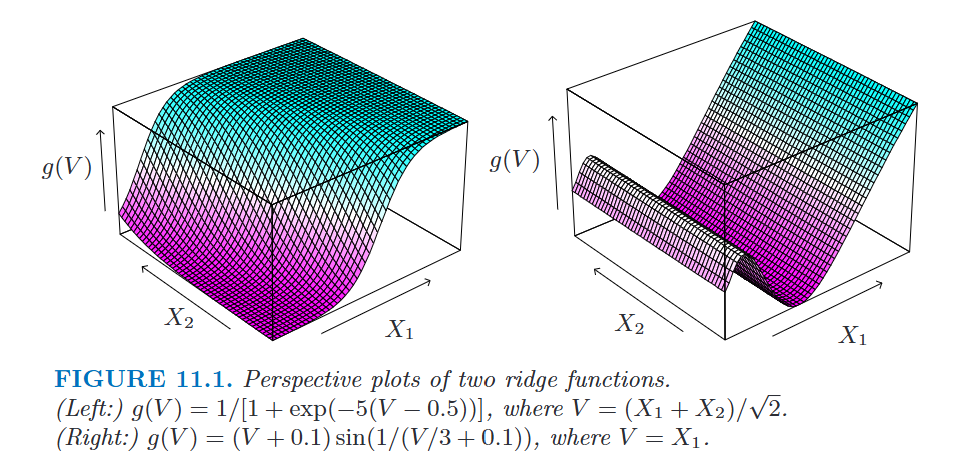
\includegraphics[width=0.95\textwidth]{Chapters/pic/ch_神经网络/figure_11_1.png}
    \caption{两个脊函数（ridge function）的透视图。\textbf{左}：$g(V) = 1/[1+\exp(-5(V-0.5))]$，其中 $V = (X_1+X_2)/\sqrt{2}$，函数只沿 $X_1+X_2$ 方向变化。\textbf{右}：$g(V) = (V+0.1)\sin(1/(V/3+0.1))$，其中 $V = X_1$。}
    \label{fig:11_1}
\end{figure}
\end{remark}

\paragraph{为什么 $g_m(\omega_m^T X)$ 只在 $\omega_m$ 定义的方向上变化？$\omega_m^T X$ 是内积吗？}

是的，$\omega_m^T X = \sum_{j=1}^p \omega_{mj} X_j = \langle \omega_m, X\rangle$ 就是标准欧氏内积（点积）。由于 $\omega_m$ 是单位向量（$\norm{\omega_m}=1$），该内积的几何意义正是 $X$ 在 $\omega_m$ 方向上的\textbf{带符号投影长度}：$\omega_m^T X = \norm{X}\cos\theta$，其中 $\theta$ 为 $X$ 与 $\omega_m$ 的夹角。

关键在于 $g_m$ 的输入是标量 $V_m = \omega_m^T X$。把 $X$ 正交分解为沿 $\omega_m$ 的分量与垂直分量 $X_\perp$（即 $\omega_m^T X_\perp = 0$）：
\[
X = (X^T\omega_m)\,\omega_m + X_\perp \quad\Longrightarrow\quad
g_m(\omega_m^T X) = g_m(X^T\omega_m),
\]
函数值\textbf{完全不依赖 $X_\perp$}。于是在垂直于 $\omega_m$ 的 $(p-1)$ 维超平面 $\{X : \omega_m^T X = c\}$ 上 $g_m$ 取常数 $g_m(c)$；只有沿 $\omega_m$ 方向移动、改变 $X^T\omega_m$ 时才变化。这正解释了图 \ref{fig:11_1}：左例 $V=(X_1+X_2)/\sqrt{2}$ 沿对角线起伏、沿 $X_1-X_2$ 方向为常数——「山脊」只沿一个方向隆起，故称脊函数。

\begin{remark}[PPR 的普遍性]
PPR 模型（\ref{eq:11_1}）非常一般：对线性组合做非线性变换能生成数量惊人的模型类。例如乘积可表示为
\[
X_1 X_2 = \frac{(X_1+X_2)^2 - (X_1-X_2)^2}{4},
\]
更高阶乘积也可类似表示。事实上，当 $M$ 任意大、$g_m$ 选择适当时，PPR 能以任意精度逼近 $\R^p$ 上的任何连续函数——这类模型称为\textbf{通用逼近器}（universal approximator）。
\end{remark}

\paragraph{$X_1X_2 = \frac{(X_1+X_2)^2 - (X_1-X_2)^2}{4}$ 里投影方向和 $g_m$ 是什么？}

这个恒等式展示了 PPR 的普遍性：一个很小的 $M=2$ 模型就能精确表示乘积这一典型的「不可加/交互」结构。逐项对应：

\begin{itemize}
\item \textbf{第一项}（方向沿对角线）：$\omega_1 = \frac{1}{\sqrt2}(1,1)^T$，$V_1 = \omega_1^T X = \frac{X_1+X_2}{\sqrt2}$，$g_1(v) = \frac12 v^2$。验证：$g_1(V_1) = \frac12 \cdot \frac{(X_1+X_2)^2}{2} = \frac{(X_1+X_2)^2}{4}$。
\item \textbf{第二项}（方向沿反对角线）：$\omega_2 = \frac{1}{\sqrt2}(1,-1)^T$，$V_2 = \omega_2^T X = \frac{X_1-X_2}{\sqrt2}$，$g_2(v) = -\frac12 v^2$。验证：$g_2(V_2) = -\frac12 \cdot \frac{(X_1-X_2)^2}{2} = -\frac{(X_1-X_2)^2}{4}$。
\end{itemize}

于是 $f(X) = g_1(\omega_1^T X) + g_2(\omega_2^T X) = X_1X_2$，这是一个 $M=2$ 的 PPR 模型。

两个要点：$g_m$ 都是二次函数 $g_m(v) = \pm\frac12 v^2$——注意这是「理想化的表示」，实际拟合中 $g_m$ 是用光滑器估计出来的，并不预设为二次。更关键的洞察是：普通 GAM（可加模型，用原始变量 $\sum_j f_j(X_j)$）\textbf{无法}表示 $X_1X_2$（没有交互项）；而 PPR 通过「先旋转到投影方向、再施加非线性」就能表示交互。这就是它比 GAM 更一般的本质——非线性的作用对象不是单个输入，而是输入的\textbf{线性组合}。

一句话：投影方向就是两个「旋转坐标轴」（对角线与反对角线），$g_m$ 是各自方向上的平方函数，两项相减恰好抵消交叉项、保留下乘积项。

\begin{remark}[代价：可解释性差]
这种普遍性的代价是：拟合模型的\textbf{解释通常很困难}，因为每个输入都以复杂、多面的方式进入模型。故 PPR 主要用于\textbf{预测}，而非产生可理解的模型。唯一的例外是 $M=1$ 情形，即计量经济学中的\textbf{单指标模型}（single index model），它比线性回归略一般，且解释方式类似。
\end{remark}

\subsection{PPR 的拟合算法}

给定训练数据 $(x_i, y_i)$，$i=1,\dots,N$，我们求误差函数的近似极小值：
\begin{equation}
\sum_{i=1}^{N} \left[ y_i - \sum_{m=1}^{M} g_m(\omega_m^T x_i) \right]^2, \label{eq:11_2}
\end{equation}
对函数 $g_m$ 和方向 $\omega_m$ 优化。与其它光滑问题一样，需对 $g_m$ 显式或隐式地施加复杂度约束以避免过拟合。

拟合采用\textbf{两阶段交替迭代}：

\begin{enumerate}
\item \textbf{给定 $\omega$ 估计 $g$}：先取 $M=1$（去掉下标）。由方向 $\omega$ 形成派生变量 $v_i = \omega^T x_i$，得到一维光滑问题，可用任意散点图光滑器（如光滑样条）估计 $g$。
\item \textbf{给定 $g$ 更新 $\omega$}：对 $\omega$ 极小化 \ref{eq:11_2}，用 Gauss--Newton 搜索（一种拟牛顿法，丢弃 Hessian 中含 $g$ 二阶导的部分）。设 $\omega^{\mathrm{old}}$ 为当前估计，由一阶 Taylor 展开
\begin{equation}
g(\omega^T x_i) \approx g(\omega_{\mathrm{old}}^T x_i) + g'(\omega_{\mathrm{old}}^T x_i)\,(\omega-\omega_{\mathrm{old}})^T x_i, \label{eq:11_3}
\end{equation}
得到
\begin{equation}
\sum_{i=1}^{N} \left[ y_i - g(\omega^T x_i) \right]^2
\approx
\sum_{i=1}^{N} g'(\omega_{\mathrm{old}}^T x_i)^2
\left[
\left( \omega_{\mathrm{old}}^T x_i + \frac{y_i - g(\omega_{\mathrm{old}}^T x_i)}{g'(\omega_{\mathrm{old}}^T x_i)} \right) - \omega^T x_i
\right]^2. \label{eq:11_4}
\end{equation}
极小化右边即：以 $\omega_{\mathrm{old}}^T x_i + \dfrac{y_i - g(\omega_{\mathrm{old}}^T x_i)}{g'(\omega_{\mathrm{old}}^T x_i)}$ 为目标、$x_i$ 为输入、权重为 $g'(\omega_{\mathrm{old}}^T x_i)^2$ 且\textbf{无截距}的最小二乘回归，得到更新后的系数 $\omega^{\mathrm{new}}$。
\end{enumerate}

两步迭代直至收敛。多 term 情形以\textbf{前向分阶段}（forward stage-wise）方式建立模型，每阶段添加一对 $(\omega_m, g_m)$。

\begin{remark}[实现细节]
\begin{itemize}
\item 原则上任何光滑方法皆可，但方便的是能提供\textbf{导数}的方法——局部回归与光滑样条很合适。
\item 每步之后可用第 9 章的\textbf{反向拟合}（backfitting）重新调整先前各步的 $g_m$；虽可能最终减少 term 数，但未必提升预测性能。
\item 通常 $\omega_m$ 不重新调整（部分为避免过多计算）。
\item term 数 $M$ 通常在前向分阶段策略中估计：当下一个 term 不能明显改善拟合时停止；也可用\textbf{交叉验证}确定 $M$。
\end{itemize}
\end{remark}

\begin{remark}[PPR 的地位]
投影寻踪思想还有很多其它应用，如密度估计，以及与 §14.7 中 ICA 的探索性投影寻踪关系。但 PPR 在统计界并未被广泛使用——也许因为 1981 年提出时其计算需求超出了当时大多数计算机的能力。然而它代表了一次重要的思想进步，并在神经网络的领域中「重生」。
\end{remark}

\paragraph{PPR 像 EM 吗？PPR 常用吗？}

\textbf{结构上像，本质上有别。} 两者都属「交替优化」（block-coordinate / alternating minimization）家族——把参数分成两块，轮流固定一块优化另一块：

\begin{itemize}
\item \textbf{交替的两块}：EM 是隐变量分布 $\leftrightarrow$ 模型参数；PPR 是函数 $g_m \leftrightarrow$ 方向 $\omega_m$。
\item \textbf{目标}：EM 极大化似然；PPR 最小化误差函数 \ref{eq:11_2}。
\item \textbf{每步闭式解}：EM 通常有；PPR 的 $g$ 用光滑器、$\omega$ 用 Gauss--Newton（数值）。
\item \textbf{单调性保证}：EM 的对数似然单调不减；PPR 无 EM 式保证（Gauss--Newton 只是近似）。
\item \textbf{动机}：EM 基于隐变量 + 极大似然，有统计理论；PPR 只是把模型拟合好的工程策略。
\end{itemize}

所以更准确地说，PPR 是\textbf{坐标下降式交替}，不是 EM——EM 的「E 步求隐变量后验」在 PPR 中没有对应物（PPR 无隐变量，两块都是直接可观测模型中的参数/函数）。真正用 EM 的对应物是第 9 章的 \textbf{HME}（专家混合）。

\textbf{PPR 并不常用。} 书中原话是「在统计领域并未被广泛使用」，原因有二：历史原因（1981 年提出时计算量超出当时机器能力）与本质局限（可解释性差，只适合预测）。它的价值在思想上：它是神经网络的「前世」（单隐层网络就是带参数化 $g_m$——sigmoid 的 PPR，见 \ref{eq:11_7}）；$M=1$ 的退化情形即\textbf{单指标模型}（single index model），计量经济学中至今有人用；投影思想在 \textbf{ICA}、密度估计中仍有应用（§14.7）。

现代视角：如今单独用 PPR（如 R 的 \texttt{stats::ppr}）的人很少，表格数据已被 XGBoost/GBM 与深度学习取代；但「非线性作用于线性组合」这个内核是现代 ML 的地基——神经网络本质上就是把 PPR 中「任意 $g_m$」换成「固定 sigmoid + 可学习参数」的产物。

% ============ §11.3 Neural Networks ============
\section{神经网络}

\begin{definition}[神经网络模型]
神经网络是\textbf{两阶段}的回归或分类模型，通常以网络图表示。对回归，一般 $K=1$，顶部只有一个输出单元 $Y_1$；但对 $K$ 类分类，顶部有 $K$ 个单元，第 $k$ 个单元建模第 $k$ 类的概率，目标 $Y_k$ 编码为 0--1 变量。

派生特征 $Z_m$ 由输入的线性组合产生，再把目标 $Y_k$ 建模为 $Z_m$ 线性组合的函数：
\begin{align}
Z_m &= \sigma(\alpha_{0m} + \alpha_m^T X), \quad m = 1,\dots,M, \nonumber \\
T_k &= \beta_{0k} + \beta_k^T Z, \quad k = 1,\dots,K, \nonumber \\
f_k(X) &= g_k(T), \quad k = 1,\dots,K, \label{eq:11_5}
\end{align}
其中 $Z=(Z_1,\dots,Z_M)$，$T=(T_1,\dots,T_K)$。
\end{definition}

\begin{figure}[htbp]
    \centering
    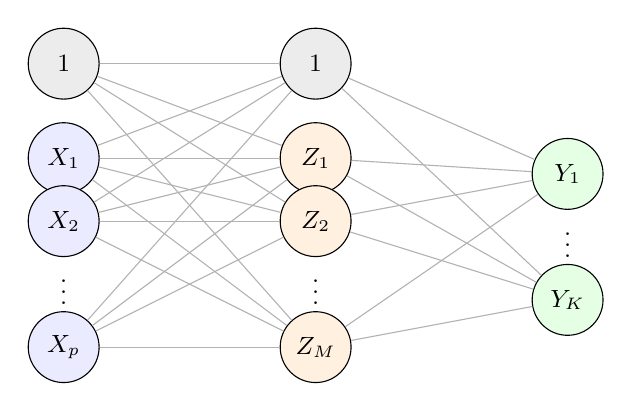
\begin{tikzpicture}[>=stealth, font=\small,
        xnode/.style={circle, draw, minimum size=9mm, inner sep=0pt, fill=blue!8},
        hnode/.style={circle, draw, minimum size=9mm, inner sep=0pt, fill=orange!12},
        ynode/.style={circle, draw, minimum size=9mm, inner sep=0pt, fill=green!10},
        bnode/.style={circle, draw, minimum size=9mm, inner sep=0pt, fill=gray!15}]
        % ---- 输入层（含偏置 X0=1）----
        \node[bnode] (X0) at (0, 1.6) {1};
        \node[xnode] (X1) at (0, 0.4)  {$X_1$};
        \node[xnode] (X2) at (0, -0.4) {$X_2$};
        \node at (0, -1.2) {$\vdots$};
        \node[xnode] (Xp) at (0, -2.0) {$X_p$};
        % ---- 隐藏层（含偏置 Z0=1）----
        \node[bnode] (Z0) at (3.2, 1.6) {1};
        \node[hnode] (Z1) at (3.2, 0.4)  {$Z_1$};
        \node[hnode] (Z2) at (3.2, -0.4) {$Z_2$};
        \node at (3.2, -1.2) {$\vdots$};
        \node[hnode] (ZM) at (3.2, -2.0) {$Z_M$};
        % ---- 输出层 ----
        \node[ynode] (Y1) at (6.4, 0.2) {$Y_1$};
        \node at (6.4, -0.6) {$\vdots$};
        \node[ynode] (YK) at (6.4, -1.4) {$Y_K$};
        % ---- 输入 → 隐藏（含偏置）----
        \foreach \a in {X0, X1, X2, Xp}
          \foreach \b in {Z0, Z1, Z2, ZM}
            \draw[gray!60] (\a) -- (\b);
        % ---- 隐藏 → 输出（含偏置）----
        \foreach \a in {Z0, Z1, Z2, ZM}
          \foreach \b in {Y1, YK}
            \draw[gray!60] (\a) -- (\b);
    \end{tikzpicture}
    \caption{单隐层前馈神经网络示意图（对应 \ref{eq:11_5}）：输入层 $X_1,\dots,X_p$ → 隐藏层 $Z_1,\dots,Z_M$ → 输出层 $Y_1,\dots,Y_K$。灰色圆为偏置单元（常数「1」），同时连到隐藏层与输出层，捕获截距 $\alpha_{0m}$ 与 $\beta_{0k}$。}
    \label{fig:11_2}
\end{figure}

\begin{remark}[激活函数与偏置]
激活函数 $\sigma(v)$ 通常取 sigmoid $\sigma(v) = 1/(1+e^{-v})$；有时也用第 6 章的高斯径向基函数作 $\sigma(v)$，得到所谓的\textbf{径向基函数网络}（RBF network）。

网络图常额外画一个「偏置单元」连到隐藏层与输出层的每个单元：把常数「1」看作额外的输入特征，该偏置单元就捕获了模型 \ref{eq:11_5} 中的截距 $\alpha_{0m}$ 与 $\beta_{0k}$。
\end{remark}

\begin{remark}[输出函数 $g_k(T)$]
$g_k(T)$ 对输出向量 $T$ 作最后的变换。回归通常取恒等 $g_k(T)=T_k$；$K$ 类分类早期也用恒等，后来改用 \textbf{softmax} 函数
\begin{equation}
g_k(T) = \frac{e^{T_k}}{\sum_{\ell=1}^{K} e^{T_\ell}}, \label{eq:11_6}
\end{equation}
这正是 §4.4 多类 logit 模型所用的变换，产生为正且和为 1 的估计。§4.2 还讨论了线性激活函数的其它问题（尤其是潜在的严重掩蔽效应）。
\end{remark}

\begin{remark}[隐藏单元 = 学习参数的基展开]
网络中间计算派生特征 $Z_m$ 的单元称为\textbf{隐藏单元}（hidden units），因为 $Z_m$ 不可直接观测。一般可有多个隐藏层。可将 $Z_m$ 看作原始输入 $X$ 的\textbf{基展开}，神经网络就是使用这些变换作为输入的线性模型（或多类 logit 模型）。与第 5 章基展开技术相比有一个重要增强：\textbf{这里基函数的参数是从数据学习的}。
\end{remark}

\begin{remark}[sigmoid 的激活行为]
图 11.3 展示了 $\sigma(v) = 1/(1+\exp(-v))$，以及 $\sigma(sv)$（$s=\frac12$ 与 $s=10$）。尺度参数 $s$ 控制激活速率：$s$ 很大时约等于在 $v=0$ 处硬激活；$\sigma(s(v-v_0))$ 把激活阈值从 0 移到 $v_0$。

若 $\sigma$ 为恒等函数，整个模型坍缩为输入的\textbf{线性模型}。故神经网络是线性模型的非线性推广。注意到 sigmoid 的激活速率取决于 $\norm{\alpha_m}$：若 $\norm{\alpha_m}$ 很小，该单元实际工作在其激活函数的线性部分。
\end{remark}

\begin{remark}[神经网络与 PPR 的关系]
单隐层神经网络与 PPR 模型形式\textbf{完全相同}，区别在于：PPR 用非参数函数 $g_m(v)$，而神经网络用基于 $\sigma(v)$ 的简单得多的函数（其参数仅 3 个）。将神经网络视为 PPR 模型：
\begin{equation}
g_m(\omega_m^T X) = \beta_m \sigma(\alpha_{0m} + \alpha_m^T X)
= \beta_m \sigma\!\left( \alpha_{0m} + \norm{\alpha_m}(\omega_m^T X) \right), \label{eq:11_7}
\end{equation}
其中 $\omega_m = \alpha_m / \norm{\alpha_m}$ 是第 $m$ 个单位向量。由于 $\sigma_{\beta,\alpha_0,s}(v) = \beta\sigma(\alpha_0 + sv)$ 比一般的非参数 $g(v)$ 复杂度低，神经网络常用 20 或 100 个这样的函数，而 PPR 通常用更少（如 $M=5$ 或 10）。
\end{remark}

\begin{remark}[名称由来]
「神经网络」源于其最初作为人脑模型而发展：每个单元代表一个神经元，连接（图中的边）代表突触。早期模型中，神经元在传入信号超过某阈值时「激发」，即 $\sigma$ 与 $g_m$ 用阶跃函数。后来神经网络被认识到是\textbf{非线性统计建模}的有用工具，而阶跃函数对优化不够光滑，故被更光滑的阈值函数（即图 11.3 的 sigmoid）取代。
\end{remark}

\begin{figure}[htbp]
    \centering
    \begin{tikzpicture}[>=stealth, font=\small,
        stage/.style={draw, rounded corners=2pt, inner sep=5pt, align=center, fill=blue!8, minimum width=6.2cm},
        feat/.style={draw, rounded corners=2pt, inner sep=5pt, align=center, fill=orange!12, minimum width=6.2cm, thick},
        outnode/.style={draw, rounded corners=2pt, inner sep=5pt, align=center, fill=green!10, minimum width=6.2cm, thick},
        note/.style={draw, rounded corners=2pt, inner sep=4pt, align=left, fill=gray!8, text width=4.6cm},
        lbl/.style={font=\small\itshape}]
        % ---- 主流程（纵向）----
        \node[stage] (X)    at (0, 0)    {输入 $X \in \R^p$};
        \node[stage] (lin1) at (0, -2.3) {线性组合（第 1 阶段）\\[1pt] $\alpha_{0m} + \alpha_m^T X$};
        \node[feat]  (Z)    at (0, -4.6) {隐藏单元（派生特征）\\[1pt] $Z_m = \sigma(\alpha_{0m} + \alpha_m^T X)$};
        \node[stage] (lin2) at (0, -6.9) {线性组合（第 2 阶段）\\[1pt] $T_k = \beta_{0k} + \beta_k^T Z$};
        \node[outnode] (f)    at (0, -9.2) {输出\\[1pt] $f_k(X) = g_k(T)$};
        % 主流程箭头
        \draw[->, thick] (X)    -- (lin1) node[midway, right, lbl] {权重 $\alpha_m$、偏置 $\alpha_{0m}$};
        \draw[->, thick] (lin1) -- (Z)    node[midway, right, lbl] {激活 $\sigma(\cdot)$};
        \draw[->, thick] (Z)    -- (lin2) node[midway, right, lbl] {权重 $\beta_k$、偏置 $\beta_{0k}$};
        \draw[->, thick] (lin2) -- (f)    node[midway, right, lbl] {$g_k$：回归恒等 / 分类 softmax};
        % ---- 右侧概念要点 ----
        \node[note] (n1) at (6.8, -2.9) {\textbf{偏置单元}：把常数「1」当额外特征，\\ 连到隐藏/输出层，捕获 $\alpha_{0m}$、$\beta_{0k}$};
        \node[note] (n2) at (6.8, -4.9) {\textbf{隐藏单元} $=$ 学习参数的\\ 基展开（对比第 5 章）};
        \node[note] (n3) at (6.8, -6.9) {\textbf{sigmoid} $\sigma(v)=\tfrac{1}{1+e^{-v}}$：\\ $s$ 大 $\to$ 硬激活；$\sigma$ 恒等 $\to$ 线性模型};
        \node[note] (n4) at (6.8, -9.2) {\textbf{与 PPR 关系}（\ref{eq:11_7}）：\\ $g_m(\omega_m^T X)=\beta_m\sigma(\alpha_{0m}+\alpha_m^T X)$};
        % 虚线连接概念
        \draw[dashed, gray] (lin1.south east) -- (n1.west);
        \draw[dashed, gray] (Z.east)           -- (n2.west);
        \draw[dashed, gray] (Z.south east)     -- (n3.west);
        \draw[dashed, gray] (f.east)           -- (n4.west);
    \end{tikzpicture}
    \caption{§11.3 神经网络概念流程：输入经\textbf{两阶段}线性组合与非线性的激活/输出得到 $f_k(X)$。右侧列出本小节的若干要点：偏置单元、隐藏单元作为学习参数的基展开、sigmoid 激活行为，以及与 PPR 的关系（\ref{eq:11_7}）。}
    \label{fig:11_3flow}
\end{figure}

% ============ §11.4 Fitting Neural Networks ============
\section{拟合神经网络}

神经网络模型的未知参数常称为\textbf{权重}（weights）。完整权重集记为 $\theta$：
\begin{equation}
\{\alpha_{0m}, \alpha_m;\, m=1,\dots,M\} \text{ 共 } M(p+1) \text{ 个权重}, \qquad
\{\beta_{0k}, \beta_k;\, k=1,\dots,K\} \text{ 共 } K(M+1) \text{ 个权重}. \label{eq:11_8}
\end{equation}

\subsection{误差函数}

对\textbf{回归}，用平方误差和作为拟合度量：
\begin{equation}
R(\theta) = \sum_{k=1}^{K} \sum_{i=1}^{N} \left( y_{ik} - f_k(x_i) \right)^2. \label{eq:11_9}
\end{equation}

对\textbf{分类}，用平方误差或交叉熵（偏差）：
\begin{equation}
R(\theta) = -\sum_{i=1}^{N} \sum_{k=1}^{K} y_{ik} \log f_k(x_i), \label{eq:11_10}
\end{equation}
对应的分类器为 $G(x) = \argmax_k f_k(x)$。

\begin{remark}[softmax + 交叉熵 = 极大似然]
使用 softmax 激活函数与交叉熵误差函数时，神经网络模型恰是隐藏单元上的\textbf{线性 logistic 回归}，所有参数均由极大似然估计得到。
\end{remark}

\begin{remark}[正则化的必要性]
我们通常\textbf{不想要} $R(\theta)$ 的全局极小，因为它很可能是过拟合解。需要某种正则化：通过惩罚项直接实现，或通过早停（early stopping）间接实现（见下一节）。
\end{remark}

\subsection{反向传播 (Back-Propagation)}

极小化 $R(\theta)$ 的通用方法是梯度下降，在此背景下称为\textbf{反向传播}。由于模型的复合结构，梯度可用链式法则轻松导出；只需对网络做一次前向、一次后向扫描，并跟踪各单元局部的量。

以平方误差损失为例详细推导。先整理推导所需的几组关系式：

\begin{remark}[推导所需的关系式]
\textbf{（1）前向传播链}（由 \ref{eq:11_5} 逐层复合）：
\begin{align}
z_{mi} &= \sigma(\alpha_{0m} + \alpha_m^T x_i), \quad m=1,\dots,M, \nonumber \\
T_{ki} &= \beta_{0k} + \beta_k^T z_i, \quad k=1,\dots,K, \nonumber \\
f_k(x_i) &= g_k(T_{ki}), \label{eq:11_11a}
\end{align}
即输入 $x_i$ 先经「线性组合 $\to$ 激活」得到隐藏单元 $z_i$，再经「线性组合 $\to$ 输出函数」得到 $f_k$。

\textbf{（2）平方误差}（\ref{eq:11_11}）：$R_i = \sum_k (y_{ik} - f_k(x_i))^2$，故 $\partial R_i/\partial f_k = -2\,(y_{ik} - f_k(x_i))$。

\textbf{（3）链式法则的两个环节}（$\beta_{km}$ 与 $\alpha_{m\ell}$ 分别影响 $f_k$ 的路径）：
\begin{align}
\frac{\partial R_i}{\partial \beta_{km}} &=
\underbrace{\frac{\partial R_i}{\partial f_k}}_{-2(y_{ik}-f_k)}
\cdot \underbrace{\frac{\partial f_k}{\partial T_{ki}}}_{g'_k(\beta_k^T z_i)}
\cdot \underbrace{\frac{\partial T_{ki}}{\partial \beta_{km}}}_{z_{mi}}, \label{eq:11_11b} \\
\frac{\partial R_i}{\partial \alpha_{m\ell}} &=
\sum_{k} \frac{\partial R_i}{\partial f_k} \frac{\partial f_k}{\partial T_{ki}} \frac{\partial T_{ki}}{\partial z_{mi}} \frac{\partial z_{mi}}{\partial \alpha_{m\ell}}, \label{eq:11_11c}
\end{align}
其中 $\partial T_{ki}/\partial z_{mi} = \beta_{km}$，$\partial z_{mi}/\partial \alpha_{m\ell} = \sigma'(\alpha_m^T x_i)\, x_{i\ell}$。注意 $\alpha_{m\ell}$ 通过单个隐藏单元 $z_{mi}$ 影响\textbf{所有} $k$ 个输出，故需对 $k$ 求和。
\end{remark}

令 $z_{mi} = \sigma(\alpha_{0m} + \alpha_m^T x_i)$（来自 \ref{eq:11_5}），$z_i = (z_{1i},\dots,z_{Mi})$，则
\begin{equation}
R(\theta) \equiv \sum_{i=1}^{N} R_i = \sum_{i=1}^{N} \sum_{k=1}^{K} \left( y_{ik} - f_k(x_i) \right)^2, \label{eq:11_11}
\end{equation}
导数为
\begin{align}
\frac{\partial R_i}{\partial \beta_{km}} &= -2\,(y_{ik} - f_k(x_i))\, g'_k(\beta_k^T z_i)\, z_{mi}, \nonumber \\
\frac{\partial R_i}{\partial \alpha_{m\ell}} &= - \sum_{k=1}^{K} 2\,(y_{ik} - f_k(x_i))\, g'_k(\beta_k^T z_i)\, \beta_{km}\, \sigma'(\alpha_m^T x_i)\, x_{i\ell}. \label{eq:11_12}
\end{align}

给定这些导数，第 $(r+1)$ 次迭代的梯度下降更新为
\begin{align}
\beta_{km}^{(r+1)} &= \beta_{km}^{(r)} - \gamma_r \sum_{i=1}^{N} \frac{\partial R_i}{\partial \beta_{km}^{(r)}}, \nonumber \\
\alpha_{m\ell}^{(r+1)} &= \alpha_{m\ell}^{(r)} - \gamma_r \sum_{i=1}^{N} \frac{\partial R_i}{\partial \alpha_{m\ell}^{(r)}}, \label{eq:11_13}
\end{align}
其中 $\gamma_r$ 是学习率。

将 \ref{eq:11_12} 改写为
\begin{equation}
\frac{\partial R_i}{\partial \beta_{km}} = \delta_{ki} z_{mi}, \qquad
\frac{\partial R_i}{\partial \alpha_{m\ell}} = s_{mi} x_{i\ell}. \label{eq:11_14}
\end{equation}
量 $\delta_{ki}$ 与 $s_{mi}$ 分别是当前模型在输出层与隐藏层单元的「误差」。由定义，它们满足
\begin{equation}
s_{mi} = \sigma'(\alpha_m^T x_i) \sum_{k=1}^{K} \beta_{km} \delta_{ki}, \label{eq:11_15}
\end{equation}
这就是所谓的\textbf{反向传播方程}。

\paragraph{反向传播方程的详细推导}

先由 \ref{eq:11_12} 第一式与 \ref{eq:11_14} 第一式对比，读出 $\delta_{ki}$ 的定义：
\[
\frac{\partial R_i}{\partial \beta_{km}} = \underbrace{-2\,(y_{ik}-f_k)\, g'_k(\beta_k^T z_i)}_{\delta_{ki}} \cdot z_{mi}.
\]
即
\begin{equation}
\delta_{ki} = -2\,(y_{ik} - f_k(x_i))\, g'_k(\beta_k^T z_i). \label{eq:11_15a}
\end{equation}

再看 \ref{eq:11_12} 第二式，把不含 $k$ 求和的因子提出来：
\[
\frac{\partial R_i}{\partial \alpha_{m\ell}}
= - \sum_{k=1}^{K} 2\,(y_{ik}-f_k)\, g'_k(\beta_k^T z_i)\, \beta_{km}\, \sigma'(\alpha_m^T x_i)\, x_{i\ell}
= \sigma'(\alpha_m^T x_i) \left[ \sum_{k=1}^{K} \beta_{km}\, \delta_{ki} \right] x_{i\ell}.
\]
与 \ref{eq:11_14} 第二式 $\partial R_i/\partial \alpha_{m\ell} = s_{mi} x_{i\ell}$ 对比，即得
\[
s_{mi} = \sigma'(\alpha_m^T x_i) \sum_{k=1}^{K} \beta_{km} \delta_{ki},
\]
这正是反向传播方程 \ref{eq:11_15}。\qed

\paragraph{公式意义}

\begin{itemize}
\item $\delta_{ki}$：\textbf{输出层}第 $k$ 个单元的误差信号。它等于「输出残差 $-2(y_{ik}-f_k)$」乘以「输出函数斜率 $g'_k$」，即该单元输出偏离目标越多、输出函数越陡，误差信号越强。
\item $s_{mi}$：\textbf{隐藏层}第 $m$ 个单元的误差信号。它等于「激活函数斜率 $\sigma'(\alpha_m^T x_i)$」乘以「所有输出层误差 $\delta_{ki}$ 经权重 $\beta_{km}$ 加权求和」。也就是说，隐藏单元的误差是从输出层\textbf{沿连接反向传播}回来的：输出层误差经权重加权、再乘本层激活导数。
\item 「反向传播」的名字由此而来：误差 $\delta_{ki}$（输出层）沿网络反向传递到隐藏层得到 $s_{mi}$，二者分别就是 \ref{eq:11_14} 中两个梯度所需的「误差」。整个计算只用到各单元\textbf{局部}的量（本单元输入、激活导数、相邻层的误差），这正是两遍算法与并行实现的依据。
\end{itemize}

\begin{figure}[htbp]
    \centering
    \begin{tikzpicture}[>=stealth, font=\small,
        inode/.style={circle, draw, minimum size=8.5mm, inner sep=0pt, fill=blue!8},
        hnode/.style={circle, draw, minimum size=8.5mm, inner sep=0pt, fill=orange!12},
        onode/.style={circle, draw, minimum size=8.5mm, inner sep=0pt, fill=green!10},
        lyr/.style={font=\bfseries\small}]
        % ---- 层标签 ----
        \node[lyr] (lx) at (-4.0, 2.7) {输入层};
        \node[lyr] (lz) at (0, 2.7)    {隐藏层};
        \node[lyr] (lf) at (4.0, 2.7)  {输出层};
        % ---- 输入层 ----
        \node[inode] (x1) at (-4.0, 1.6) {$x_1$};
        \node[inode] (x2) at (-4.0, 0.5) {$x_2$};
        \node at (-4.0, -0.25) {$\vdots$};
        \node[inode] (xl) at (-4.0, -1.0) {$x_p$};
        \node[align=center, gray] at (-4.0, -2.1) {输入值 $x_{i\ell}$};
        % ---- 隐藏层 ----
        \node[hnode] (z1) at (0, 1.6) {$z_1$};
        \node[hnode] (z2) at (0, 0.5) {$z_2$};
        \node at (0, -0.25) {$\vdots$};
        \node[hnode] (zm) at (0, -1.0) {$z_M$};
        \node[align=center, gray] at (0, -2.1) {$z_{mi} = \sigma(\alpha_{0m}+\alpha_m^T x_i)$};
        \node[align=center, red] at (0, -3.0) {误差 $s_{mi} = \sigma'(\alpha_m^T x_i)\sum_k \beta_{km}\delta_{ki}$};
        % ---- 输出层 ----
        \node[onode] (f1) at (4.0, 1.6) {$f_1$};
        \node at (4.0, 0.85) {$\vdots$};
        \node[onode] (fk) at (4.0, 0.1) {$f_K$};
        \node[align=center, gray] at (4.0, -1.5) {$f_k = g_k(T_{ki})$};
        \node[align=center, red] at (4.0, -2.4) {误差 $\delta_{ki}$};
        % ---- 前向连接（灰色实线）----
        \foreach \a in {x1,x2,xl}
          \foreach \b in {z1,z2,zm}
            \draw[gray!60] (\a) -- (\b);
        \foreach \a in {z1,z2,zm}
          \foreach \b in {f1,fk}
            \draw[gray!60] (\a) -- (\b);
        % ---- 反向传播（红色虚线箭头）----
        \draw[red, dashed, thick, ->] (f1.south west) -- (z1.north east) node[midway, above, red, sloped, font=\scriptsize] {$\delta_{1i}$};
        \draw[red, dashed, thick, ->] (fk.west) -- (zm.east) node[midway, below, red, sloped, font=\scriptsize] {$\delta_{Ki}$};
        \draw[red, dashed, ->] (z1.west) -- (x1.east) node[midway, above, red, sloped, font=\scriptsize] {$s_{1i}$};
        \draw[red, dashed, ->] (zm.west) -- (xl.east) node[midway, below, red, sloped, font=\scriptsize] {$s_{Mi}$};
    \end{tikzpicture}
    \caption{前向传播（灰色实线）与反向传播（红色虚线）中各量在网络中的对应位置：输入层存放输入值 $x_{i\ell}$；隐藏层由 $z_{mi}=\sigma(\alpha_{0m}+\alpha_m^T x_i)$ 生成派生特征，并接收反传误差 $s_{mi}$；输出层由 $f_k=g_k(T_{ki})$ 给出预测并计算误差 $\delta_{ki}$。反向传播把输出层误差 $\delta_{ki}$ 沿连接传回隐藏层得到 $s_{mi}$（\ref{eq:11_15}）。}
    \label{fig:11_4bp}
\end{figure}

\begin{remark}[两遍算法]
利用上述方程，更新 \ref{eq:11_13} 可用两遍算法实现：
\begin{itemize}
\item \textbf{前向传播}：固定当前权重，用 \ref{eq:11_5} 计算预测值 $\hat{f}_k(x_i)$。
\item \textbf{后向传播}：计算误差 $\delta_{ki}$，再经 \ref{eq:11_15} 反传得到隐藏层误差 $s_{mi}$。
\end{itemize}
两组误差再经 \ref{eq:11_14} 用于计算 \ref{eq:11_13} 中的梯度。反向传播也称 \textbf{delta 规则}（Widrow \& Hoff, 1960）。交叉熵的计算组件与平方误差同形（见习题 11.3）。
\end{remark}

\begin{remark}[反向传播的优点]
反向传播的优点在于\textbf{简单、局部}：每个隐藏单元只与共享连接的单元传递信息，因此可在并行架构计算机上高效实现。
\end{remark}

\subsection{Batch 学习与在线学习}

更新 \ref{eq:11_13} 是一种\textbf{batch 学习}——参数更新是所有训练样本的和。学习也可\textbf{在线}进行：逐个处理观测，每处理一个样本就更新梯度，并多遍循环训练样本；此时 \ref{eq:11_13} 中的求和退化为单一项。一个\textbf{epoch}（回合）指完整扫过训练集一遍。在线学习让网络能处理非常大的训练集，也能随新观测到来增量更新权重。

\begin{remark}[学习率 $\gamma_r$]
batch 学习的学习率 $\gamma_r$ 通常取常数，也可用线搜索每次更新时极小化误差函数来优化。在线学习中 $\gamma_r$ 应随迭代 $r\to\infty$ 趋于 0。这是一种\textbf{随机近似}（Robbins--Munro, 1951）：若 $\gamma_r\to 0$、$\sum_r \gamma_r = \infty$、$\sum_r \gamma_r^2 < \infty$（例如 $\gamma_r = 1/r$）则保证收敛。
\end{remark}

\begin{remark}[反向传播可能很慢]
反向传播可能非常慢，因而通常不是首选方法。牛顿法等二阶方法也不合适，因为 $R$ 的 Hessian 可能非常大。更好的拟合方法包括\textbf{共轭梯度}与\textbf{变度量}（variable metric）方法，它们避免显式计算二阶导矩阵，同时收敛更快。
\end{remark}

% ============ §11.5 Some Issues in Training Neural Networks ============
\section{训练神经网络的若干问题}

训练神经网络颇有「艺术」成分：模型通常\textbf{过参数化}，优化问题\textbf{非凸}且不稳定，除非遵循某些准则。

\subsection{起始值 (Starting Values)}

\begin{remark}[从小权重随机起始]
若权重接近 0，sigmoid 的有效部分近似线性，网络便坍缩为近似线性模型。通常起始权重取接近 0 的随机值，于是模型从近似线性开始，随权重增大而变非线性：各单元在需要处局部化到某些方向并引入非线性。使用\textbf{精确的 0 权重}会导致零导数与完全对称，算法永不移动；从大权重开始则常得到差解。
\end{remark}

\subsection{过拟合 (Overfitting)}

神经网络常有太多权重，会在 $R$ 的全局极小处过拟合。早期（有意或无意地）用\textbf{早停}（early stopping）规则避免过拟合：只训练一段时间，远未接近全局极小前停止。由于权重从高正则化（线性）解出发，这等价于把最终模型向线性模型\textbf{收缩}。用验证集确定停止时刻——预期验证误差开始上升时停止。

更显式的正则化是\textbf{权重衰减}（weight decay），类比线性模型的岭回归（§3.4.1）：在误差函数上加惩罚 $R(\theta) + \lambda J(\theta)$，其中
\begin{equation}
J(\theta) = \sum_{k,m} \beta_{km}^2 + \sum_{m,\ell} \alpha_{m\ell}^2, \label{eq:11_16}
\end{equation}
$\lambda \ge 0$ 是调参参数。$\lambda$ 越大，权重越被收缩向 0；通常用交叉验证估计 $\lambda$。惩罚的效果是分别给梯度表达式 \ref{eq:11_13} 加上 $2\beta_{km}$ 与 $2\alpha_{m\ell}$ 项。

还有其它形式的惩罚，例如
\begin{equation}
J(\theta) = \sum_{k,m} \frac{\beta_{km}^2}{1+\beta_{km}^2} + \sum_{m,\ell} \frac{\alpha_{m\ell}^2}{1+\alpha_{m\ell}^2}, \label{eq:11_17}
\end{equation}
称为\textbf{权重消除}（weight elimination）惩罚，它对较小的权重比 \ref{eq:11_16} 收缩更多。

\begin{remark}[图 11.4 / 11.5]
图 11.4 展示了对第 2 章 mixture 例训练含 10 个隐藏单元的网络，无权重衰减（上）与有权重衰减（下）的结果——权重衰减明显改善了预测。图 11.5 是估计权重的热图（其灰度版本称为 Hinton 图），可见权重衰减抑制了两层权重，使权重较均匀地分布在 10 个隐藏单元上。
\end{remark}

\subsection{输入的缩放 (Scaling of the Inputs)}

输入的缩放决定了底层权重的有效缩放，因而对最终模型质量有很大影响。最好把所有输入\textbf{标准化}为均值 0、标准差 1，这确保所有输入在正则化过程中被\textbf{平等对待}，也便于为随机起始权重选取有意义的范围。对标准化后的输入，通常取 $[-0.7, +0.7]$ 上的随机均匀权重。

\subsection{隐藏单元数与层数 (Number of Hidden Units and Layers)}

一般来说，隐藏单元\textbf{过多好于过少}：过少则模型灵活性不足，无法捕捉数据中的非线性；过多则多余权重可在合适的正则化下被收缩向 0。典型隐藏单元数在 \textbf{5 到 100} 之间，随输入数与训练样本数增加。最常见的做法是放置一个相当大的单元数并用正则化训练；有些研究者用交叉验证估计最优单元数，但若已用交叉验证估计正则化参数，这似乎没有必要。

隐藏层数的选择由背景知识与实验指导。每层都提取输入的特征（用于回归或分类）；使用多层可以构建\textbf{不同分辨率的层次化特征}。§11.6 给出有效使用多层的例子。

\subsection{多重极小 (Multiple Minima)}

误差函数 $R(\theta)$ 是\textbf{非凸}的，有大量局部极小，因此最终解很依赖起始权重的选择。至少应尝试多个随机起始配置，并选（惩罚）误差最低的解。更好的做法是：用这一组网络的\textbf{平均预测}作为最终预测（Ripley, 1996）——它优于\textbf{平均权重}，因为模型的非线性意味着平均权重解可能很差。另一种方法是\textbf{bagging}：对训练数据的随机扰动版本训练网络，再平均其预测（见 §8.7）。

% ============ §11.6 Example: Simulated Data ============
\section{模拟数据例子 (Example: Simulated Data)}

从两个加性误差模型 $Y = f(X) + \varepsilon$ 生成数据：

\begin{itemize}
\item \textbf{sigmoid 和}：$Y = \sigma(a_1^T X) + \sigma(a_2^T X) + \varepsilon_1$，其中 $a_1=(3,3)$、$a_2=(3,-3)$，$p=2$；
\item \textbf{径向函数}：$Y = \prod_{m=1}^{10} \varphi(X_m) + \varepsilon_2$，其中 $\varphi(t) = (2\pi)^{-1/2} e^{-t^2/2}$，$p=10$。
\end{itemize}

$X_j$ 为标准高斯变量。两个模型都取高斯误差，使信噪比
\begin{equation}
\frac{\Var(E(Y|X))}{\Var(Y - E(Y|X))} = \frac{\Var(f(X))}{\Var(\varepsilon)} \label{eq:11_18}
\end{equation}
为 4。训练样本 100，测试样本 10{,}000。用带权重衰减、不同隐藏单元数的网络拟合，对 10 个随机起始权重记录平均测试误差 $E_{\mathrm{Test}}(Y-\hat{f}(X))^2$。

\begin{remark}[结论]
\textbf{零隐藏单元}模型即线性最小二乘回归。神经网络完美适合 sigmoid 和模型：两单元模型表现最好，接近 Bayes 率（回归的 Bayes 率即误差方差）。但随着隐藏单元增多过拟合迅速出现，有些起始权重下甚至比线性模型更差——即使两隐藏单元，10 个起始配置中也有 2 个不比线性模型好，印证了\textbf{多起始值}的重要性。

径向函数对神经网络是最难的：它球对称、无偏好方向。图 11.6 右面板显示其测试误差远高于 Bayes 率（注意纵轴刻度与左面板不同）——事实上常数拟合（样本均值）的相对误差为 5（信噪比 4 时），可见网络比均值还差。
\end{remark}

\paragraph{脊函数和径向函数的定义分别是什么？}

\textbf{脊函数}（ridge function）：设 $g:\R\to\R$ 是任意标量函数，$\omega\in\R^p$ 为固定（通常单位）向量，称
\[
f(X) = g(\omega^T X)
\]
为 $\R^p$ 上的脊函数——它把 $p$ 维输入先投影到一维方向 $\omega$，再施加一维非线性。其等值面是垂直于 $\omega$ 的\textbf{超平面族}，即只在 $\omega$ 方向上变化。例如神经网络的单个隐藏单元 $\sigma(\alpha_0+\omega^T X)$、图 11.1 右例 $\sin(X_1)$ 都是脊函数。

\textbf{径向函数}（radial function）：设 $h:\R_{\ge 0}\to\R$ 是任意标量函数，$c\in\R^p$ 为固定中心，称
\[
f(X) = h(\|X-c\|)
\]
为以 $c$ 为中心的径向函数——它只依赖于 $X$ 到中心 $c$ 的欧氏距离，其等值面是以 $c$ 为球心的\textbf{球面族}（各向同性）。例如高斯核 $\exp(-\frac{1}{2\lambda}\|X-c\|^2)$（RBF 网络的隐藏单元）、第 5 章的薄板样条基 $r^2\log r$，以及书中的 $e^{-\|X\|^2/2}$（$c=0$）都是径向函数。

\begin{remark}[两者的对偶关系]
\begin{itemize}
\item 脊函数的等值面是\textbf{超平面族}，径向函数的等值面是\textbf{球面族}；它们都把 $p$ 维输入压缩成一个一维量再非线性化，差别在于这个一维量是「某方向上的坐标」还是「到中心的距离」。
\item 代表方法互补：脊函数对应神经网络、PPR；径向函数对应 RBF 网络、核方法、高斯过程。
\item 用 $L$ 个脊函数逼近球对称函数，所需 $L$ 随维度 $p$ \textbf{指数增长}；反之用 $L$ 个径向函数逼近脊函数也低效。两者的擅长领域互补。
\end{itemize}
\end{remark}

\paragraph{为什么球对称径向函数对神经网络不友好？能否通过更换 sigmoid 来提升？}

\textbf{结构不匹配是根本原因。} 径向函数可化简为
\[
\prod_{m=1}^{10}\varphi(X_m) = (2\pi)^{-5}\exp\!\Big(-\tfrac12\textstyle\sum_{m=1}^{10} X_m^2\Big) = (2\pi)^{-5}e^{-\frac12\|X\|^2},
\]
它只依赖 $\|X\|^2$——在所有方向上均匀变化、没有偏好方向。而神经网络每个隐藏单元 $Z_m=\sigma(\alpha_{0m}+\alpha_m^T X)$ 是\textbf{脊函数}：只在方向 $\alpha_m$ 上变化，在垂直于 $\alpha_m$ 的超平面上是常数，即每个单元只「看」一个方向。目标函数在每个方向都要变化，而每个单元只能贡献一个方向的信息，要在所有方向上逼近球对称函数就需覆盖单位球面 $S^{p-1}$ 上（连续无穷多的）所有方向——离散化后单元数随维度指数增长。对比 sigmoid 和模型 $Y=\sigma(a_1^T X)+\sigma(a_2^T X)$，方向 $a_1=(3,3)$、$a_2=(3,-3)$ 恰是网络要学的方向，两个单元就能精确表达——网络「天生」匹配这种有稀疏偏好方向的结构。

\textbf{能否通过换掉 sigmoid 提升？——取决于换成什么。} 换成另一个\textbf{脊函数}（tanh、ReLU、swish…）不能：它们仍是「线性组合 $+$ 一维非线性」，每个单元仍只对应一个方向，$p=10$ 维球对称的核心困难原封不动——改变激活函数的\textbf{形状}无法改变单元只贡献一维方向信息这一\textbf{结构}事实。但若换成\textbf{径向基函数（RBF）激活}（以距离为输入的高斯核 $Z_m=\exp(-\frac{1}{2\lambda}\|X-c_m\|^2)$，即 §11.3 提到的 RBF 网络），则能大幅提升：此时每个单元本身\textbf{球对称}，以中心 $c_m$ 为球心向所有方向衰减，天然匹配 $e^{-\|X\|^2/2}$ 的结构，只需少量 $c_m$ 就能很好地表示球对称函数。

\begin{remark}[现代视角]
脊函数族与径向函数族分别擅长对方的「盲区」。这解释了为何深度学习用卷积等\textbf{结构先验}（对图像，局部方向结构比全空间对称更重要），以及为何\textbf{高斯过程/核方法}在光滑函数回归上仍强大——它们本质上是把「方向结构」先验换成了「光滑性」先验。
\end{remark}

\begin{remark}[正则化的作用]
本例固定权重衰减 $\lambda = 0.0005$（温和正则化）。图 11.7 显示：无权重衰减时隐藏单元越多过拟合越严重；而 $\lambda = 0.1$ 对所有隐藏单元数都得到好结果，无明显过拟合。图 11.8 对 10 隐藏单元网络扫描权重衰减参数，$\lambda = 0.1$ 近似最优。

\textbf{总结}：有两个自由参数需选择——权重衰减 $\lambda$ 与隐藏单元数 $M$。学习策略可以是：把其中一个固定在最不受约束的值（此处为零权重衰减、10 隐藏单元），确保模型足够丰富，再用\textbf{交叉验证}选择另一个。对比图 11.7 与图 11.8 可见测试误差对 $\lambda$ 不如对 $M$ 敏感，故优先交叉验证 $\lambda$。
\end{remark}

% ============ §11.7 Example: ZIP Code Data ============
\section{ZIP 码数据例子 (Example: ZIP Code Data)}

这是手写数字识别的字符分类任务，曾在 ML 与神经网络界多年作为基准问题。图 11.9 展示了从信封自动扫描、经反倾斜与尺寸归一化后的 $16\times 16$ 灰度数字图像（Le Cun et al., 1990）；这 256 个像素值作为分类器的输入。

纯黑箱神经网络并不理想地适合此任务，部分因为像素表示缺乏某些不变性（如小幅旋转）。早期尝试的误分类率约 4.5%。本节展示为克服这些缺陷而\textbf{手工设计}网络的先驱工作（Le Cun, 1989），最终推动了神经网络性能的最先进水平（Le Cun et al., 1998）。

为使效果突出，样本量刻意取得很小：训练集 320 个数字、测试集 160 个（并加随机水平平移生成额外图像）。拟合了五个不同的网络：

\begin{description}
\item[Net-1] 无隐藏层，等价于\textbf{多项 logistic 回归}（256 输入 → 10 个输出单元，对应数字 0--9）。
\item[Net-2] 单隐藏层、12 个隐藏单元、全连接（前述标准网络）。
\item[Net-3] 两个隐藏层、\textbf{局部连接}（locally connected）。
\item[Net-4] 两个隐藏层、局部连接 + \textbf{权重共享}。
\item[Net-5] 两个隐藏层、局部连接、\textbf{两级权重共享}。
\end{description}

所有网络用 sigmoid 输出单元与平方误差函数拟合。由于参数多于训练观测，所有网络训练误差均为 0%；测试误差随训练 epoch 的演化见图 11.11：线性网络 Net-1 很快过拟合，其余网络在越来越优的水平上趋于平稳。

\begin{remark}[局部连接与卷积网络]
\textbf{局部连接}：每个隐藏单元只连到下一层的一小块（patch）。Net-3 第一隐藏层为 $8\times 8$ 阵列，每个单元取输入层 $3\times 3$ 块的输入；第二隐藏层取 $5\times 5$ 块。这使每个单元负责从下层提取局部特征，并大幅减少权重总数——Net-3 比 Net-2 隐藏单元更多，但连接/权重更少（1226 vs.\ 3214），性能相近。

\textbf{权重共享}（Net-4/Net-5）：同一局部特征图（feature map）内所有单元在图像不同位置执行同一操作——共享同一组权重。Net-4 第一隐藏层有两个 $8\times 8$ 阵列，每个单元取 $3\times 3$ 块，但同一特征图内各单元共享同一组 9 个权重（各保留自己的偏置）。这迫使图像不同部分用\textbf{同一线性泛函}提取特征，这类网络即所谓的\textbf{卷积网络}（convolutional network）。共享权重关于 $R$ 的梯度等于该权重控制的各条连接梯度之和。
\end{remark}

\begin{table}[htbp]
\centering
\caption{五个网络在手写数字分类上的测试表现（Le Cun, 1989）。}
\label{tab:11_1}
\begin{tabular}{lcccc}
\toprule
网络 & 架构 & 连接数 & 权重数 & 正确率 \\
\midrule
Net-1 & 单层网络 & 2570 & 2570 & 80.0\% \\
Net-2 & 两层网络 & 3214 & 3214 & 87.0\% \\
Net-3 & 局部连接 & 1226 & 1226 & 88.5\% \\
Net-4 & 约束网络 1 & 2266 & 1132 & 94.0\% \\
Net-5 & 约束网络 2 & 5194 & 1060 & 98.4\% \\
\bottomrule
\end{tabular}
\end{table}

\begin{remark}[结果与启示]
Net-4 连接数多于 Net-3 但权重数更少，测试性能更优；Net-5 第二隐藏层有 4 个 $4\times 4$ 特征图，各连 $5\times 5$ 局部块且共享权重，误差仅 1.6\%——远优于标准网络 Net-2 的 13\%。Net-5 的巧妙设计源于「手写风格的特征应出现在数字的多处」这一先验，是多年实验的产物。它说明\textbf{神经网络并非全自动工具}：和所有统计模型一样，领域知识应当被用来改进性能。

该网络后来被\textbf{切线距离}方法（Simard et al., 1993，§13.3.3）超越。至 1998 年，在大数据集（NIST，60{,}000 训练 / 10{,}000 测试）上报告的最佳错误率：切线距离 + 1-NN 1.1\%、9 次多项式 SVM 0.8\%、更复杂的卷积网络 LeNet-5 0.8\%、boosted LeNet-4 0.7\%。误差估计的标准误约 0.1\%（$N=10{,}000$、$p\approx 0.01$ 的二项平均），故误差率相差 0.1--0.2\% 内统计等价；实际标准误更高，因为测试数据已被隐式用于调参。
\end{remark}

% ============ §11.8 Discussion ============
\section{讨论 (Discussion)}

PPR 与神经网络都是对输入的线性组合（「派生特征」）取非线性函数。这是回归与分类非常强大而一般的途径，在许多问题上可与最好的学习方法竞争。

\begin{remark}[适用场景与局限]
这些工具在\textbf{高信噪比}、以\textbf{预测（而非解释）}为目标的问题中尤其有效；在需要描述产生数据的物理过程、解释各输入作用的问题中则较弱——每个输入以非线性方式、在多处进入模型。Hinton (1989) 曾把进入每个隐藏单元的估计权重画成图来理解各单元提取的特征，但这受限于参数向量的\textbf{不可识别性}：常有 $\alpha_m$ 张成同一线性空间的解给出几乎相同的预测。有人建议对这些权重做主成分分析以寻找可解释解。总体而言，可解释性困难限制了其在医学等重视解释领域的应用。

另一方面，与 CART、MARS 等方法不同，神经网络是\textbf{实值参数的平滑函数}，这为贝叶斯推断提供了便利——下一节讨论一个成功的贝叶斯实现。
\end{remark}

% ============ §11.9 Bayesian Neural Nets and the NIPS 2003 Challenge ============
\section{贝叶斯神经网络与 NIPS 2003 挑战}

2003 年举行了一个分类竞赛：向参赛者提供五个已标注的二分类训练集（不同规模、来自不同领域，见表 11.2），并可用验证集特征在网站上提交预测（12 周反馈期），最后用联合训练+验证集训练后对独立测试集提交最终预测。共 75 组参赛，20/16 组提交验证/测试结果。竞赛强调特征提取，数据中加入人工「探针」——与真实特征分布相似但与类别标签无关的噪声特征（各数据集探针比例见表 11.2），算法须自行识别并降权或剔除。

评估指标包括测试集正确率、ROC 曲线下面积、以及两两分类器直接比较的综合分。结果（Guyon et al., 2006）中最重要的发现：\textbf{Neal \& Zhang (2006) 的参赛条目是明显总冠军}——在五个数据集上三个第一，另两个分别第 5、第 7。其胜出条目用一系列预处理特征选择步骤，之后接\textbf{贝叶斯神经网络}、Dirichlet 扩散树及其组合。

\begin{table}[htbp]
\centering
\caption{NIPS 2003 挑战数据集。$p$ 为特征数（Dorothea 的特征为二值），$N_{\mathrm{tr}}, N_{\mathrm{val}}, N_{\mathrm{te}}$ 分别为训练/验证/测试样本数。}
\label{tab:11_2}
\begin{tabular}{lclccccc}
\toprule
数据集 & 领域 & 特征类型 & $p$ & 探针比例 & $N_{\mathrm{tr}}$ & $N_{\mathrm{val}}$ & $N_{\mathrm{te}}$ \\
\midrule
Arcene & 质谱 & 稠密 & 10{,}000 & 30\% & 100 & 100 & 700 \\
Dexter & 文本分类 & 稀疏 & 20{,}000 & 50\% & 300 & 300 & 2{,}000 \\
Dorothea & 药物发现 & 稀疏 & 100{,}000 & 50\% & 800 & 350 & 800 \\
Gisette & 数字识别 & 稠密 & 5{,}000 & 30\% & 6{,}000 & 1{,}000 & 6{,}500 \\
Madelon & 人工 & 稠密 & 500 & 96\% & 2{,}000 & 600 & 1{,}800 \\
\bottomrule
\end{tabular}
\end{table}

\subsection{Bayes、Boosting 与 Bagging}

先简要回顾贝叶斯推断及其在神经网络上的应用。给定训练数据 $(X^{\mathrm{tr}}, y^{\mathrm{tr}})$ 与参数 $\theta$ 的采样模型，Neal \& Zhang (2006) 使用双隐层神经网络，输出节点为二分类的类概率 $\Pr(Y\mid X,\theta)$。给先验 $\Pr(\theta)$，参数后验为
\begin{equation}
\Pr(\theta\mid X^{\mathrm{tr}}, y^{\mathrm{tr}}) = \frac{\Pr(\theta)\, \Pr(y^{\mathrm{tr}}\mid X^{\mathrm{tr}},\theta)}{\int \Pr(\theta)\, \Pr(y^{\mathrm{tr}}\mid X^{\mathrm{tr}},\theta)\, d\theta}. \label{eq:11_19}
\end{equation}
对测试样本 $(X^{\mathrm{new}}, Y^{\mathrm{new}})$，预测分布为
\begin{equation}
\Pr(Y^{\mathrm{new}}\mid X^{\mathrm{new}}, X^{\mathrm{tr}}, y^{\mathrm{tr}}) = \int \Pr(Y^{\mathrm{new}}\mid X^{\mathrm{new}},\theta)\, \Pr(\theta\mid X^{\mathrm{tr}}, y^{\mathrm{tr}})\, d\theta. \label{eq:11_20}
\end{equation}

由于 \ref{eq:11_20} 的积分不可处理，用成熟的 \textbf{MCMC} 方法从后验采样：生成数百个 $\theta$ 值，简单平均即估计积分。Neal \& Zhang (2006) 对所有参数用弥散高斯先验，采用的 MCMC 叫\textbf{混合蒙特卡洛}（hybrid Monte Carlo）：引入辅助动量向量、实现以目标密度为势函数的哈密顿动力学，从而避免随机游走行为——连续候选点以更大步长在样本空间移动、相关性更低、收敛更快。

\paragraph{HMC 的严格数学定理}

设目标分布 $\pi(\theta) \propto e^{-U(\theta)}$，势能 $U(\theta) = -\log\pi(\theta)$。HMC 引入辅助动量 $p\in\R^d$ 与动能 $K(p)=\tfrac12 p^T M^{-1}p$（$M$ 为对称正定质量矩阵），构造相空间联合分布
\[
\pi(\theta,p) \propto e^{-H(\theta,p)}, \qquad H(\theta,p) = U(\theta) + K(p),
\]
其 $\theta$ 边际恰为 $\pi(\theta)$（因为 $\int e^{-K(p)}dp$ 与 $\theta$ 无关）。哈密顿动力学
\[
\dot\theta = \frac{\partial H}{\partial p} = M^{-1}p, \qquad
\dot p = -\frac{\partial H}{\partial \theta} = -\nabla U(\theta) = \nabla\log\pi(\theta)
\]
具有三个关键性质：
\begin{enumerate}
\item \textbf{能量守恒}：$\frac{d}{dt}H(\theta(t),p(t)) = 0$（沿轨道 $H$ 不变）；
\item \textbf{体积守恒}（Liouville 定理）：相空间体积在动力学流下不变，即映射保测；
\item \textbf{时间可逆}：$p\to-p$ 后轨道反向，动力学可逆。
\end{enumerate}

数值实现用 \textbf{leapfrog（蛙跳）}积分，步长 $\epsilon$、共 $L$ 步：
\begin{align}
p_{t+\epsilon/2} &= p_t - \tfrac{\epsilon}{2}\nabla U(\theta_t), \nonumber \\
\theta_{t+\epsilon} &= \theta_t + \epsilon\, M^{-1} p_{t+\epsilon/2}, \nonumber \\
p_{t+\epsilon} &= p_{t+\epsilon/2} - \tfrac{\epsilon}{2}\nabla U(\theta_{t+\epsilon}). \label{eq:11_20a}
\end{align}
蛙跳是\textbf{辛}（symplectic）积分器：保持体积、可逆，能量误差 $O(\epsilon^2)$ 且有界。

\begin{theorem}[HMC 的正确性]
设 $\epsilon$ 固定，leapfrog 映射 $\mathcal{T}_\epsilon:(\theta,p)\mapsto(\theta^*,p^*)$ 是双射、可逆且保体积。以
\[
\alpha = \min\Bigl(1,\; e^{-[H(\theta^*,p^*)-H(\theta,p)]}\Bigr)
\]
为接受概率的 Metropolis 校正，使马尔可夫链以 $\pi(\theta,p)\propto e^{-H(\theta,p)}$ 为\textbf{唯一不变分布}，其 $\theta$ 边际即目标 $\pi(\theta)$。由于 leapfrog 的能量误差有界且 $O(\epsilon^2)$，接受率可维持在较高水平。
\end{theorem}

\begin{remark}[为何 HMC 比随机游走 MH 快]
随机游走 MH 的候选点在高维下扩散缓慢、相邻样本自相关高；HMC 沿能量守恒轨道大步滑动、相邻样本相关性低，有效样本量更大。代价是需计算梯度 $\nabla U(\theta)=\nabla\log\pi(\theta)$——故仅适用于光滑可微的目标（如神经网络后验），对不光滑模型（如树）不适用（呼应 §11.9 末尾的结论）。
\end{remark}

\begin{remark}[HMC 与模拟退火 (SA) 的关系]
两者都借用统计物理的「能量 + 温度」语言：目标写成玻尔兹曼形式 $\pi(\theta)\propto e^{-E(\theta)/T}$。但目的不同——\textbf{HMC 固定温度（$T=1$）用于高效采样}（估计后验期望），\textbf{SA 则随时间降低温度 $T$ 用于优化}（找 $\arg\min E(\theta)$）。SA 本质是「带温度调度的 Metropolis」：高温时大范围探索、低温时收敛到低能态；HMC 本质是「带动量/动力学的 Metropolis」：用哈密顿轨道代替随机游走提议。二者可结合（如并行回火/退火 HMC），在高维多模态分布上同时利用温度跨越与动力学加速。
\end{remark}

\paragraph{贝叶斯神经网络的形式化定义}

\begin{definition}[贝叶斯神经网络 (Bayesian Neural Network, BNN)]
贝叶斯神经网络 = \textbf{神经网络骨架} + \textbf{贝叶斯推断外壳}。设网络输出为 $f_k(X;\theta)$（如二分类的类概率 $\Pr(Y\mid X,\theta)$），权重 $\theta$ 不再是单一的点估计，而视为服从后验分布 $\Pr(\theta\mid X^{\mathrm{tr}},y^{\mathrm{tr}})$（\ref{eq:11_19}）的随机变量。\textbf{输入}与普通神经网络完全相同（特征向量 $X$）；\textbf{输出}是预测分布 $\Pr(Y^{\mathrm{new}}\mid X^{\mathrm{new}},X^{\mathrm{tr}},y^{\mathrm{tr}})$（\ref{eq:11_20}），而非单点预测——因此天然携带不确定性。
\end{definition}

\paragraph{BNN 的四步流程}

\begin{enumerate}
\item \textbf{建模}：设定采样模型（似然）与先验：
\[
\Pr(y^{\mathrm{tr}}\mid X^{\mathrm{tr}},\theta) = \prod_{i=1}^{N} \Pr(y_i\mid x_i,\theta) \quad(\text{网络给出类概率}), \qquad \Pr(\theta)\ (\text{弥散高斯先验}).
\]

\item \textbf{推断}：由贝叶斯公式求权重的联合后验（\ref{eq:11_19}）：
\[
\Pr(\theta\mid X^{\mathrm{tr}}, y^{\mathrm{tr}}) = \frac{\Pr(\theta)\, \Pr(y^{\mathrm{tr}}\mid X^{\mathrm{tr}},\theta)}{\int \Pr(\theta)\, \Pr(y^{\mathrm{tr}}\mid X^{\mathrm{tr}},\theta)\, d\theta} \propto \Pr(\theta)\, \Pr(y^{\mathrm{tr}}\mid X^{\mathrm{tr}},\theta).
\]
注意是整个参数向量 $\theta=(\alpha,\beta)$ 共用一个\textbf{联合}后验，而非每个权重各自独立；分母为归一化常数。

\item \textbf{采样}：后验积分不可解析，用 MCMC（此处为 HMC）从后验分布采样出数百个权重样本 $\theta_1,\dots,\theta_L$，用经验分布近似后验：
\[
\Pr(\theta\mid X^{\mathrm{tr}}, y^{\mathrm{tr}}) \;\approx\; \frac{1}{L}\sum_{\ell=1}^{L} \delta(\theta - \theta_\ell), \qquad \theta_\ell \sim \Pr(\theta\mid X^{\mathrm{tr}}, y^{\mathrm{tr}}).
\]
每次采样都同时移动所有权重，但目的不是「收敛到一个最优」，而是「遍历后验分布」。

\item \textbf{预测}：把后验近似代入预测分布 \ref{eq:11_20}，将积分换成对样本平均（\ref{eq:11_21} 取 $w_\ell=1/L$）：
\[
\Pr(Y^{\mathrm{new}}\mid X^{\mathrm{new}}, X^{\mathrm{tr}}, y^{\mathrm{tr}})
= \int \Pr(Y^{\mathrm{new}}\mid X^{\mathrm{new}},\theta)\, \Pr(\theta\mid X^{\mathrm{tr}}, y^{\mathrm{tr}})\, d\theta
\;\approx\; \frac{1}{L}\sum_{\ell=1}^{L} \Pr(Y^{\mathrm{new}}\mid X^{\mathrm{new}},\theta_\ell).
\]
即对每个采样权重计算预测概率，再\textbf{简单平均}得到最终预测分布——这正是贝叶斯模型平均（Bayesian Model Averaging）。
\end{enumerate}

\paragraph{弥散高斯先验 (diffuse Gaussian prior)}

\begin{definition}[弥散高斯先验]
弥散（diffuse）= 对参数\textbf{几乎没有先验信息}。弥散高斯先验就是\textbf{中心在 0、方差取很大的高斯分布}，作为每个权重的先验：
\[
\Pr(\theta_j) = \mathcal{N}(\theta_j \mid 0, \sigma_0^2), \qquad \sigma_0^2 \text{ 很大}, \qquad \Pr(\theta) = \prod_j \mathcal{N}(\theta_j \mid 0, \sigma_0^2),
\]
其中 $\sigma_0^2$ 相对参数的合理尺度取很大值，使得这个钟形曲线极宽极平，在感兴趣的区间内几乎处处接近均匀分布。
\end{definition}

\textbf{为什么用高斯？} 高斯密度光滑、处处可微——后验因此光滑可微，保证 HMC 所需的梯度 $\nabla_\theta\log\pi(\theta)$ 存在。这正是「HMC 只适用光滑模型」这一要求在选择先验时的体现。

\textbf{为什么弥散（方差大）？} 因为 $e^{-\theta_j^2/2\sigma_0^2}$ 在 $\sigma_0^2$ 很大时、于参数合理范围内几乎恒等于 1——先验几乎不改变后验形状，后验基本由似然决定，让数据说了算。有限但很大的 $\sigma_0^2$ 等价于一个\textbf{极弱的 $L_2$（岭式）先验}；若 $\sigma_0^2\to\infty$ 则退化为不严格归一化的无信息均匀先验。

\textbf{与 ARD 的关系}：§11.9 后面的 ARD 是弥散高斯先验的精细化——不再让所有权重共用一个大方差 $\sigma_0^2$，而是给\textbf{每个特征} $j$ 一个独立的先验方差 $\sigma_j^2$（均值仍 0），再看后验中 $\sigma_j^2$ 是否被数据压得很小：若后验方差集中在很小的值，说明该特征不重要，可丢弃。即 ARD = 逐特征的弥散高斯先验 + 用后验方差做特征筛选。

\begin{remark}[普通 NN 与 BNN 的对比]
\begin{center}
\begin{tabular}{lcc}
\toprule
 & 普通神经网络 & 贝叶斯神经网络 \\
\midrule
权重 & 一个 $\hat\theta$（点估计） & 后验分布 $\Pr(\theta\mid \text{data})$ \\
迭代目的 & 收敛到最优 & 遍历后验（采样） \\
最终产物 & 一个训练好的网络 & 数百个权重样本 \\
输出 & 点预测 $\hat f(X)$ & 预测分布（含不确定性） \\
过拟合处理 & 正则化 / 早停 & 后验平均自动处理 \\
代价 & 快 & 慢（需采多个权重） \\
\bottomrule
\end{tabular}
\end{center}
\end{remark}

特征预处理尝试两种形式：
\begin{enumerate}
\item 用 $t$ 检验做\textbf{单变量筛选}（univariate screening）；
\item \textbf{自动相关判定}（ARD）：第 $j$ 个特征到第一隐藏层各单元的权重共享共同先验方差 $\sigma_j^2$、先验均值 0，计算各 $\sigma_j^2$ 的后验，丢弃后验方差集中在很小值的特征。
\end{enumerate}

\paragraph{ARD 的全称与定义}

\textbf{ARD} = \textbf{Automatic Relevance Determination}（自动相关判定）。它给\textbf{每个特征} $j$ 一个独立的先验方差 $\sigma_j^2$（先验均值 0），通过贝叶斯推断计算各 $\sigma_j^2$ 的\textbf{后验分布}，然后丢弃那些后验方差集中在很小值的特征。

\textbf{工作原理}：先验设特征 $j$ 到第一隐藏层各单元的权重共享 $\mathcal{N}(0,\sigma_j^2)$——「特征 $j$ 的相关性」由它自己的方差 $\sigma_j^2$ 控制。贝叶斯推断后，若数据里特征 $j$ 对预测无关紧要，后验会把 $\sigma_j^2$ \textbf{压得很小}（等价于把该特征权重强烈收缩到 0）。于是看每个 $\sigma_j^2$ 的后验：后验方差集中在很小值 $\Rightarrow$ 该特征「自动判定为不相关」，可丢弃。即 ARD 让数据自己决定每个特征该保留多少。

\textbf{公式化表达}。设特征 $j$ 到第一隐藏层的权重为 $\theta_{j\cdot}=(\theta_{j1},\dots,\theta_{jM})$，ARD 的层级模型为
\begin{align}
\theta_{jm} \mid \sigma_j^2 &\sim \mathcal{N}(0, \sigma_j^2), \quad m=1,\dots,M \ (\text{共享先验方差}), \nonumber \\
\sigma_j^2 &\sim \text{Inv-Gamma}(a, b) \quad (\text{超先验, 或经验贝叶斯点估计}), \label{eq:11_21a}
\end{align}
于是「特征 $j$ 的相关性」由 $\sigma_j^2$ 一个超参数统一控制。对特征 $j$ 的权重做边际化后，其后验为
\begin{equation}
\Pr(\sigma_j^2 \mid \text{data}) \;\propto\; \Pr(\sigma_j^2) \int \Pr(\text{data}\mid \theta) \prod_{m=1}^{M}\mathcal{N}(\theta_{jm}\mid 0,\sigma_j^2)\, d\theta_{j\cdot}. \label{eq:11_21b}
\end{equation}
\textbf{判定准则}：若 $\Pr(\sigma_j^2\mid \text{data})$ 集中在很小的 $\sigma_j^2$ 处，则特征 $j$ 的权重后验被强烈收缩向 0，判定该特征不相关并丢弃。

\textbf{与弥散高斯先验的关系}：弥散高斯先验是\textbf{所有特征共用}一个大方差 $\sigma_0^2$；ARD 是\textbf{逐特征}独立方差 $\sigma_j^2$ 的精细化——ARD = 逐特征的弥散高斯先验 + 用后验方差做特征筛选。

\paragraph{筛选特征集与 ARD 缩减特征集}

这是 §11.9.2 性能比较中使用的\textbf{两种不同的特征预处理结果}：

\begin{center}
\begin{tabular}{lcc}
\toprule
 & 筛选特征集 & ARD 缩减特征集 \\
\midrule
所用方法 & 单变量 $t$ 检验 & ARD（贝叶斯） \\
特征是否独立 & 每个特征独立筛 & 由模型后验决定 \\
是否需要模型 & 不需要（纯统计检验） & 需先拟合贝叶斯网络 \\
\bottomrule
\end{tabular}
\end{center}

\textbf{关键区别}：筛选特征集对每个特征单独做 $t$ 检验（看其在两类间是否有显著差异），完全不依赖任何模型，是「自洽」的预处理；ARD 缩减特征集由贝叶斯神经网络的 ARD 后验方差决定，\textbf{隐含地用了贝叶斯网络的推断结果}。

\textbf{为何重要}：因为 ARD 缩减特征集「来自贝叶斯神经网络方法」，故对比时只有用筛选特征集的方法才是\textbf{自洽、完整}的流程——非贝叶斯方法（boosted trees、random forests 等）若用 ARD 缩减特征集，等于「借用」了贝叶斯方法的信息，对它们不公平。这也正是作者强调「只有使用筛选特征集的方法才是 legitimate、self-contained procedures」的原因。

\begin{remark}[成功要素与贝叶斯的真正力量]
该方法有三个可能重要的特征：(a) 特征选择与预处理、(b) 神经网络模型、(c) 用 MCMC 的贝叶斯推断。据 Neal \& Zhang (2006)，(a) 中的特征筛选\textbf{纯为计算效率}——特征多时 MCMC 很慢；避免过拟合无需特征选择，因为后验平均 \ref{eq:11_20} 会自动处理。

作者观点：现代贝叶斯方法的力量\textbf{不在于作为正式推断程序}（很少有人真信高维复杂神经网络中的先验是正确的），而在于它给出一种\textbf{高效采样模型空间相关部分、再对高概率模型的预测做平均}的方式。

Bagging 与 boosting 是非贝叶斯方法，但与贝叶斯模型中的 MCMC 有相似性。贝叶斯方法固定数据、按当前后验估计扰动参数；bagging 以 i.i.d.\ 方式扰动数据再重估模型得到新参数；boosting 类似 bagging，但拟合的是各基学习器模型的加和，且用非 i.i.d.\ 样本学习。这些都可写为
\begin{equation}
\hat{f}(x^{\mathrm{new}}) = \sum_{\ell=1}^{L} w_\ell\, \E(Y^{\mathrm{new}}\mid x^{\mathrm{new}}, \hat{\theta}_\ell). \label{eq:11_21}
\end{equation}
其中 $\hat{\theta}_\ell$ 是大批模型参数。贝叶斯：$w_\ell = 1/L$，从后验采样 $\theta_\ell$ 估计后验均值；bagging：$w_\ell = 1/L$，$\hat{\theta}_\ell$ 是 bootstrap 重采样重拟合的参数；boosting：权重全为 1，但 $\hat{\theta}_\ell$ 以非随机、顺序方式选择以持续改进拟合。
\end{remark}

\subsection{性能比较}

基于上述相似性，在表 11.2 的五个数据集上比较了贝叶斯神经网络、boosted 树、boosted 神经网络、随机森林与 bagged 神经网络。细节：贝叶斯网络为双隐层 20 与 8 单元（Neal 的 C 包）；boosted 树用 R 的 gbm（每轮 bag 80\% 数据，shrinkage 0.001--0.1，树深 2--9）；boosted 神经网络用 2 或 4 单元单隐层网络（nnet）；随机森林用默认参数；bagged 网络与贝叶斯网络同架构。

\begin{remark}[结果]
图 11.12 与表 11.3 显示，使用筛选特征集与 ARD 缩减特征集时，\textbf{贝叶斯神经网络再次胜出}，但对某些数据集差异统计不显著（误差条宽度为一个标准误）。随机森林在筛选特征集上表现最好，boosted 神经网络在缩减特征集上最好、几乎赶上贝叶斯网络。

boosted 神经网络优于 boosted 树，说明神经网络模型更适合这些问题：单个特征可能不是好的预测器，而\textbf{特征的线性组合效果更好}；但随机森林的出色表现与此解释相悖（出乎作者意料）。由于缩减特征集来自贝叶斯方法，只有用筛选特征集的方法才是自洽的完整流程。表 11.3 同时显示非贝叶斯方法在计算时间上有明显优势。

总体而言，贝叶斯神经网络的优势可能来自：(a) 神经网络模型很适合这五个问题，(b) MCMC 高效探索了参数空间的重要部分并按质量平均模型。贝叶斯方法对\textbf{平滑参数化}的模型（如神经网络）有效；对不光滑的模型（如树）是否同样有效尚不清楚。
\end{remark}

\begin{table}[htbp]
\centering
\caption{不同方法的性能：五个问题上测试误差的平均排名（低为好）及平均计算时间（分钟，括号内为标准误）。}
\label{tab:11_3}
\begin{tabular}{lcccc}
\toprule
& \multicolumn{2}{c}{筛选特征} & \multicolumn{2}{c}{ARD 缩减特征} \\
\cmidrule(lr){2-3}\cmidrule(lr){4-5}
方法 & 平均排名 & 平均时间 & 平均排名 & 平均时间 \\
\midrule
贝叶斯神经网络 & 1.5 & 384 (138) & 1.6 & 600 (186) \\
Boosted 树 & 3.4 & 3.0 (2.5) & 4.0 & 34.1 (32.4) \\
Boosted 神经网络 & 3.8 & 9.4 (8.6) & 2.2 & 35.6 (33.5) \\
随机森林 & 2.7 & 1.9 (1.7) & 3.2 & 11.2 (9.3) \\
Bagged 神经网络 & 3.6 & 3.5 (1.1) & 4.0 & 6.4 (4.4) \\
\bottomrule
\end{tabular}
\end{table}

% ============ §11.10 Computational Considerations ============
\section{计算考虑 (Computational Considerations)}

对 $N$ 个观测、$p$ 个预测变量、$M$ 个隐藏单元、$L$ 个训练 epoch，一次神经网络拟合通常需要 $O(NpML)$ 次运算。可用于拟合神经网络的软件包非常多（可能远多于主流统计方法的包），但质量参差；由于神经网络的学习问题对输入缩放等问题敏感，应\textbf{仔细选择并测试}这类软件。

% ============ 本章小结 ============
\section{本章小结}

\subsection{核心框架}

\begin{figure}[H]
    \centering
    \begin{tikzpicture}[
        node distance=1.1cm and 1.5cm,
        inode/.style={draw, rounded corners, fill=blue!8, text width=3.0cm, align=center, minimum height=0.9cm, font=\small},
        hnode/.style={draw, rounded corners, fill=orange!12, text width=3.4cm, align=center, minimum height=0.9cm, font=\small},
        onode/.style={draw, rounded corners, fill=green!10, text width=3.0cm, align=center, minimum height=0.9cm, font=\small},
        freqbox/.style={draw, rounded corners, fill=cyan!8, text width=3.4cm, align=center, minimum height=1.0cm, font=\footnotesize},
        bayesbox/.style={draw, rounded corners, fill=purple!10, text width=3.4cm, align=center, minimum height=1.0cm, font=\footnotesize},
        tipbox/.style={draw, rounded corners, fill=gray!8, text width=3.0cm, align=center, minimum height=1.0cm, font=\footnotesize},
        arrow/.style={->, >=stealth, thick},
        darrow/.style={->, >=stealth, dashed, thick}
    ]
        % ---- 第一行：模型主线 ----
        \node[inode] (X)  at (0, 0)    {输入\\ $X \in \R^p$};
        \node[hnode] (Z)  at (6, 0)  {隐藏单元（派生特征）\\ $Z_m = \sigma(\alpha_{0m}+\alpha_m^T X)$};
        \node[onode] (F)  at (12, 0)  {输出\\ $f_k(X) = g_k(T_k)$\\ 恒等 / softmax};
        \draw[arrow] (X) -- (Z) node[midway, above, font=\scriptsize] {线性组合 + $\sigma$};
        \draw[arrow] (Z) -- (F) node[midway, above, font=\scriptsize] {线性组合 + $g_k$};

        % ---- 第二行：训练（反向传播 + 正则化）----
        \node[freqbox] (bp) at (2.0, -2.6) {拟合：反向传播\\ 前向+后向扫描、链式法则、$\delta_{ki}\to s_{mi}$};
        \node[freqbox] (reg) at (8.0, -2.6) {正则化：\\ 权重衰减 / 早停 / 权重消除};
        \draw[darrow] (Z.south) -- (bp.north);
        \draw[darrow] (F.south) -- (reg.north);
        \draw[arrow] (bp) -- (reg) node[midway, above, font=\scriptsize] {防止过拟合};

        % ---- 第三行：训练技巧 ----
        \node[tipbox] (tip) at (4.2, -5.2) {训练技巧\\ 多随机起始值 $\cdot$ 输入标准化\\ $\cdot$ 隐藏单元 5--100 $\cdot$ 多重极小};
        \draw[arrow] (reg) -- (tip);

        % ---- 第四行：贝叶斯扩展 ----
        \node[bayesbox] (post) at (0.0, -7.8) {贝叶斯神经网络\\ $\Pr(\theta\mid \text{data})$ \eqref{eq:11_19}};
        \node[bayesbox] (hmc)  at (6.0, -7.8) {HMC 采样\\ $\theta_1,\dots,\theta_L \sim$ 后验};
        \node[bayesbox] (avg)  at (12.0, -7.8) {后验平均预测\\ $\frac{1}{L}\sum_\ell \Pr(Y\mid X,\theta_\ell)$};
        \draw[darrow, purple] (tip.south) -- (post.north);
        \draw[arrow, purple] (post) -- (hmc) node[midway, above, font=\scriptsize] {动量+梯度};
        \draw[arrow, purple] (hmc) -- (avg) node[midway, above, font=\scriptsize] {模型平均};
        \node[below=0.25cm of avg, font=\footnotesize, purple] {ARD 特征筛选};
    \end{tikzpicture}
    \caption{第 11 章核心框架：神经网络是\textbf{脊函数的叠加}（输入线性组合 + 非线性激活 → 派生特征 → 输出函数），用\textbf{反向传播}拟合、\textbf{正则化}防过拟合；进一步可用\textbf{贝叶斯}方式把权重视为后验分布，用 \textbf{HMC} 采样并做\textbf{后验平均}预测。}
    \label{fig:11_summary}
\end{figure}

\subsection{要点回顾}

\begin{itemize}
\item \textbf{模型本质}：神经网络是「脊函数」的叠加，与 PPR 形式相同、只是把非参数 $g_m$ 换成参数化的 sigmoid 函数；它是线性模型的非线性推广，参数化的基函数从数据学习。
\item \textbf{拟合}：最小化误差函数（回归用平方误差、分类用交叉熵）$\to$ 反向传播（两遍算法，误差从输出层反传到隐藏层）$\to$ 梯度下降更新权重。
\item \textbf{训练艺术}：小随机起始值、输入标准化、权重衰减/早停、隐藏单元数 5--100、多起始值应对多重极小——误差函数非凸，训练需要这些准则。
\item \textbf{适用性}：适合高信噪比、以预测为目标的问题；可解释性差（每个输入多处非线性进入），不擅长描述物理机制。
\item \textbf{结构先验}：ZIP 码例子展示用局部连接 + 权重共享（\textbf{卷积网络}）把领域知识编码进架构，可大幅提升性能（Net-5 错误率 1.6\% vs.\ 全连接 13\%）。
\item \textbf{贝叶斯扩展}：把权重当作随机变量，求后验 $\Pr(\theta\mid\text{data})$，用 HMC 从后验采样并做后验平均——自动处理过拟合、给出不确定性；ARD 用逐特征先验方差做特征筛选。
\end{itemize}

\begin{remark}[一章主线]
从 PPR 的「非线性作用于线性组合」出发，神经网络把这一思想变成可微、可训练的两阶段模型；反向传播解决「怎么学」，正则化与训练技巧解决「学过头」，贝叶斯视角解决「学多少才可信」。
\end{remark}
